%% USPSC-TCC-modelo-ICMCe.tex
%----------------------------------------------------------------
%% Esta é uma customização do abntex2-modelo-trabalho-academico.tex de v-1.9.5 laurocesar 
%% Este trabalho utiliza a classe USPSC (USPSC.cls e USPSC1.cls) que é mantida
%% Os modelos desenvolvidos utilizam diversos arquivos relacionado em
%% 2.1 Pacote USPSC: Classe USPSC e modelos de trabalhos acadêmicos	do Tutorial do Pacote 
%%  USPSC para modelos de trabalhos de acadêmicos em LaTeX - versão 3.2

%% Sobre a classe abntex2.cls:
%% abntex2.cls, v-1.9.5 laurocesar
%% Copyright 2012-2015 by abnTeX2 group at https://www.abntex.net.br/ 
%----------------------------------------------------------------

\documentclass[
    12pt,        % tamanho da fonte
    openright,    % capítulos começam em pág ímpar (insere página vazia caso preciso)
    twoside,  % para impressão em anverso (frente) e verso. Oposto a oneside - Nota: utilizar \imprimirfolhaderosto*
%oneside, % para impressão em páginas separadas (somente anverso) -  Nota: utilizar \imprimirfolhaderosto
    a4paper,            % tamanho do papel.
% -- opções da classe abntex2 --
    chapter=TITLE,        % títulos de capítulos convertidos em letras maiúsculas
% -- opções do pacote babel --
    english,            % idioma adicional para hifenização
    french,                % idioma adicional para hifenização
    spanish,            % idioma adicional para hifenização
    brazil                % o último idioma é o principal do documento
% {class/USPSC} configura o cabeçalho contendo apenas o número da página
]{class/USPSC}
%]{class/USPSC1} %- páginas ímpares: com seções ou subseções e o número da página e páginas pares: com o número da página e o título do capítulo

% Pacotes básicos - Fundamentais
\usepackage[T1]{fontenc}        % Seleção de códigos de fonte.
\usepackage[utf8]{inputenc}        % Codificação do documento (conversão automática dos acentos)
\usepackage{lmodern}            % Usa a fonte Latin Modern
%\usepackage{times}		    	% Usa a fonte Times New Roman
% Para usar a fonte , lembre-se de tirar a % do comando %\renewcommand{\ABNTEXchapterfont}{\rmfamily}, localizado mais abaixo, logo após "Outras opções para nota de rodapé no Sistema Numérico" 					
\usepackage{lastpage}            % Usado pela Ficha catalográfica
\usepackage{indentfirst}        % Indenta o primeiro parágrafo de cada seção.
\usepackage{color}                % Controle das cores
\usepackage{graphicx}            % Inclusão de gráficos
\usepackage{float}                % Fixa tabelas e figuras no local exato
\usepackage{tikz}
\usetikzlibrary{positioning}
\usepackage{microtype}            % para melhorias de justificação
\usepackage{pdfpages}
\usepackage{makeidx}            % para gerar índice remissivo
\usepackage{hyphenat}          % Pacote para retirar a hifenizacao DO TEXTO
\usepackage[absolute]{textpos} % Pacote permite o posicionamento do texto
\usepackage{eso-pic}           % Pacote para incluir imagem de fundo
\usepackage{makebox}           % Pacote para criar caixa de texto
\usepackage{amsmath}
\usepackage{amsfonts}
\usepackage{mathtools}
\usepackage{algorithm}
\usepackage{algpseudocode}
\usepackage{siunitx}
\usepackage{hyperref}

% Pacotes de citações
% Citações padrão ABNT
% Sistemas de chamada: autor-data ou numérico.
% Sistema autor-data
% \usepackage[alf, abnt-emphasize=bf, abnt-thesis-year=both, abnt-repeated-author-omit=no, abnt-last-names=abnt, abnt-etal-cite=3, abnt-etal-list=3, abnt-etal-text=it, abnt-and-type=e, abnt-doi=doi, abnt-url-package=none, abnt-verbatim-entry=no]{abntex2cite}
% \bibliographystyle{class/abntex2-alf-USPSC}

% Se o idioma for o inglês
% \bibliographystyle{class/abntex2-alfeng-USPSC}

% Sistema Numérico
% Para citações numéricas, sistema adotado pelo IFSC, incluir % no início dos comandos acima e retirar a % dos comandos abaixo

\usepackage{cite}              % agrupa citações numéricas consecutivas
\usepackage[num, abnt-emphasize=bf, abnt-thesis-year=both, abnt-repeated-author-omit=no, abnt-last-names=abnt, abnt-etal-cite=3, abnt-etal-list=3, abnt-etal-text=it, abnt-and-type=e, abnt-doi=doi, abnt-url-package=none, abnt-verbatim-entry=no]{abntex2cite}
% \bibliographystyle{class/abntex2-num-USPSC}

% Se o idioma for o inglês, exclua % no comando acima ou do comando abaixo
\bibliographystyle{class/abntex2-numeng-USPSC}

% Há diversa opções para nota de rodapé no Sistema Numérico.  Para o IFSC, habilitade o comando abaixo.
\renewcommand{\thefootnote}{\fnsymbol{footnote}}  %Comando para inserção de símbolos em nota de rodapé

% oopções para nota de rodapé no Sistema Numérico:
%\renewcommand{\thefootnote}{\alph{footnote}}      %Comando para inserção de letras minúscula em nota de rodapé
%\renewcommand{\thefootnote}{\Alph{footnote}}      %Comando para inserção de letras maiúscula em nota de rodapé
%\renewcommand{\thefootnote}{\roman{footnote}}     %Comando para inserção de números romanos minúsculos  em nota de rodapé
%\renewcommand{\thefootnote}{\Roman{footnote}}     %Comando para inserção de números romanos minúsculos  em nota de rodapé

\renewcommand{\footnotesize}{\small} %Comando para diminuir a fonte das notas de rodapé
%Para utilizar a fonte Times New Roman, inclua retire % do início do comando abaixo 
%\renewcommand{\ABNTEXchapterfont}{\rmfamily}

% Quando for adotado o Sistema Numérico, habilite
%\usepackage[superscript]{cite}

% Pacotes adicionais, usados apenas no âmbito do Modelo Canônico do abnteX2
\usepackage{lipsum}                % para geração de dummy text

% pacotes de tabelas
\usepackage{multicol}    % Suporte a mesclagens em colunas
\usepackage{multirow}    % Suporte a mesclagens em linhas
\usepackage{longtable}    % Tabelas com várias páginas
\usepackage{threeparttablex}    % notas no longtable
\usepackage{array}

% Compatibilização com a ABNT NBR 6023:2018 e 10520:2023
\usepackage{class/ABNT6023-10520}
% As demais compatibilizações estão nos arquivos abntex2-alf-USPSC.bst,abntex2-alfeng-USPSC.bst, abntex2-num-USPSC.bst e abntex2-numeng-USPSC.bst, dependendo do idioma do textos e se o sistemas de chamada for autor-data ou numérico, conforme explicitado acima.
\usepackage{standalone}
% ---
% DADOS INICIAIS - Define sigla com título, área de concentração e opção do Programa 

% Os demais dados deverão ser fornecidos no arquivo USPSC-TCC-pre-textual-ICMC

% Configurações de aparência do PDF final
% alterando o aspecto da cor azul
\definecolor{blue}{RGB}{41,5,195}

% informações do PDF
\makeatletter
\hypersetup{
%pagebackref=true,
    pdftitle={\@title},
    pdfauthor={\@author},
    pdfsubject={\imprimirpreambulo},
    pdfcreator={LaTeX with abnTeX2},
    pdfkeywords={abnt}{latex}{abntex}{USPSC}{trabalho acadêmico},
    colorlinks=true,            % false: boxed links; true: colored links
    linkcolor=black,            % color of internal links
    citecolor=black,                % color of links to bibliography
    filecolor=black,            % color of file links
    urlcolor=black,
%linkcolor=blue,            	% color of internal links
%citecolor=blue,        		% color of links to bibliography
%filecolor=magenta,      		% color of file links
%urlcolor=blue,
    bookmarksdepth=4
}
\makeatother

\renewcommand{\subsectionautorefname}{Subsection}

\siglaunidade{ICMC-TCC}
\programa{BCCe}


% Espaçamentos entre linhas e parágrafos

% O tamanho do parágrafo é dado por:
\setlength{\parindent}{1.3cm}

% Controle do espaçamento entre um parágrafo e outro:
\setlength{\parskip}{0.2cm}  % tente também \onelineskip

% compila o sumário e índice
\makeindex

% Início do documento
\begin{document}

% Seleciona o idioma do documento (conforme pacotes do babel)
%\selectlanguage{brazil}
    \selectlanguage{english}

% Retira espaço extra obsoleto entre as frases.
    \frenchspacing

% --- Formatação dos Títulos
    \renewcommand{\ABNTEXchapterfontsize}{\fontsize{12}{12}\bfseries}
    \renewcommand{\ABNTEXsectionfontsize}{\fontsize{12}{12}\bfseries}
    \renewcommand{\ABNTEXsubsectionfontsize}{\fontsize{12}{12}\normalfont}
    \renewcommand{\ABNTEXsubsubsectionfontsize}{\fontsize{12}{12}\normalfont}
    \renewcommand{\ABNTEXsubsubsubsectionfontsize}{\fontsize{12}{12}\normalfont}

% ----------------------------------------------------------
% ELEMENTOS PRÉ-TEXTUAIS
% ----------------------------------------------------------

% Capa
%imprimircapa

%Capa do ICMC
    %% USPSC-CapaICMC.tex
\AddToShipoutPicture{\BackgroundPic}
%-------------
\begin{minipage}[c]{144mm}
   \centering
   \begin{textblock*}{144mm}(61mm,65mm)
   \vspace*{1,2cm}
   \linespread{0.5}
   \ABNTEXchapterfont\bfseries\Large
   \textcolor{capa-azul}{\nohyphens{\imprimirtitulo}}
   \end{textblock*}
\end{minipage}
\vfill
\vspace*{5cm}
\begin{minipage}[t][65mm][t]{125mm}
   \begin{textblock*}{130mm}(81mm,123mm)
      \ABNTEXchapterfont\bfseries\Large
      \textcolor{capa-azul}{\nohyphens{\imprimirautor}} 
      \vfill
      \vspace{9pt}
      \ABNTEXsubsectionfontsize\small
      \renewcommand{\ABNTEXsubsectionfontsize}{\fontsize{10}{6}\normalfont}
      \ABNTEXsubsectionfontsize 
      \textcolor{capa-azul}{\nohyphens{\imprimirnotacapaicmc}}
      \renewcommand{\ABNTEXsubsectionfontsize}{\fontsize{12}{12}\normalfont}
   \end{textblock*}	
\end{minipage} 
% ---

    \AddToShipoutPicture{\BackgroundBranco}

% 
\includepdf{pretextual/USPSC-PaginaEmBranco.pdf}
    \pagebreak

% Folha de rosto do ICMC (o * indica impressão em anverso (frente) e verso )
%\imprimirfolharostocar
%\imprimirfolharostocar*

% Folha de rosto padrão do Pacote USPSC (o * indica impressão em anverso (frente) e verso )
%\imprimirfolhaderosto
    \imprimirfolhaderosto*

% Inserir a ficha catalográfica em pdf
% 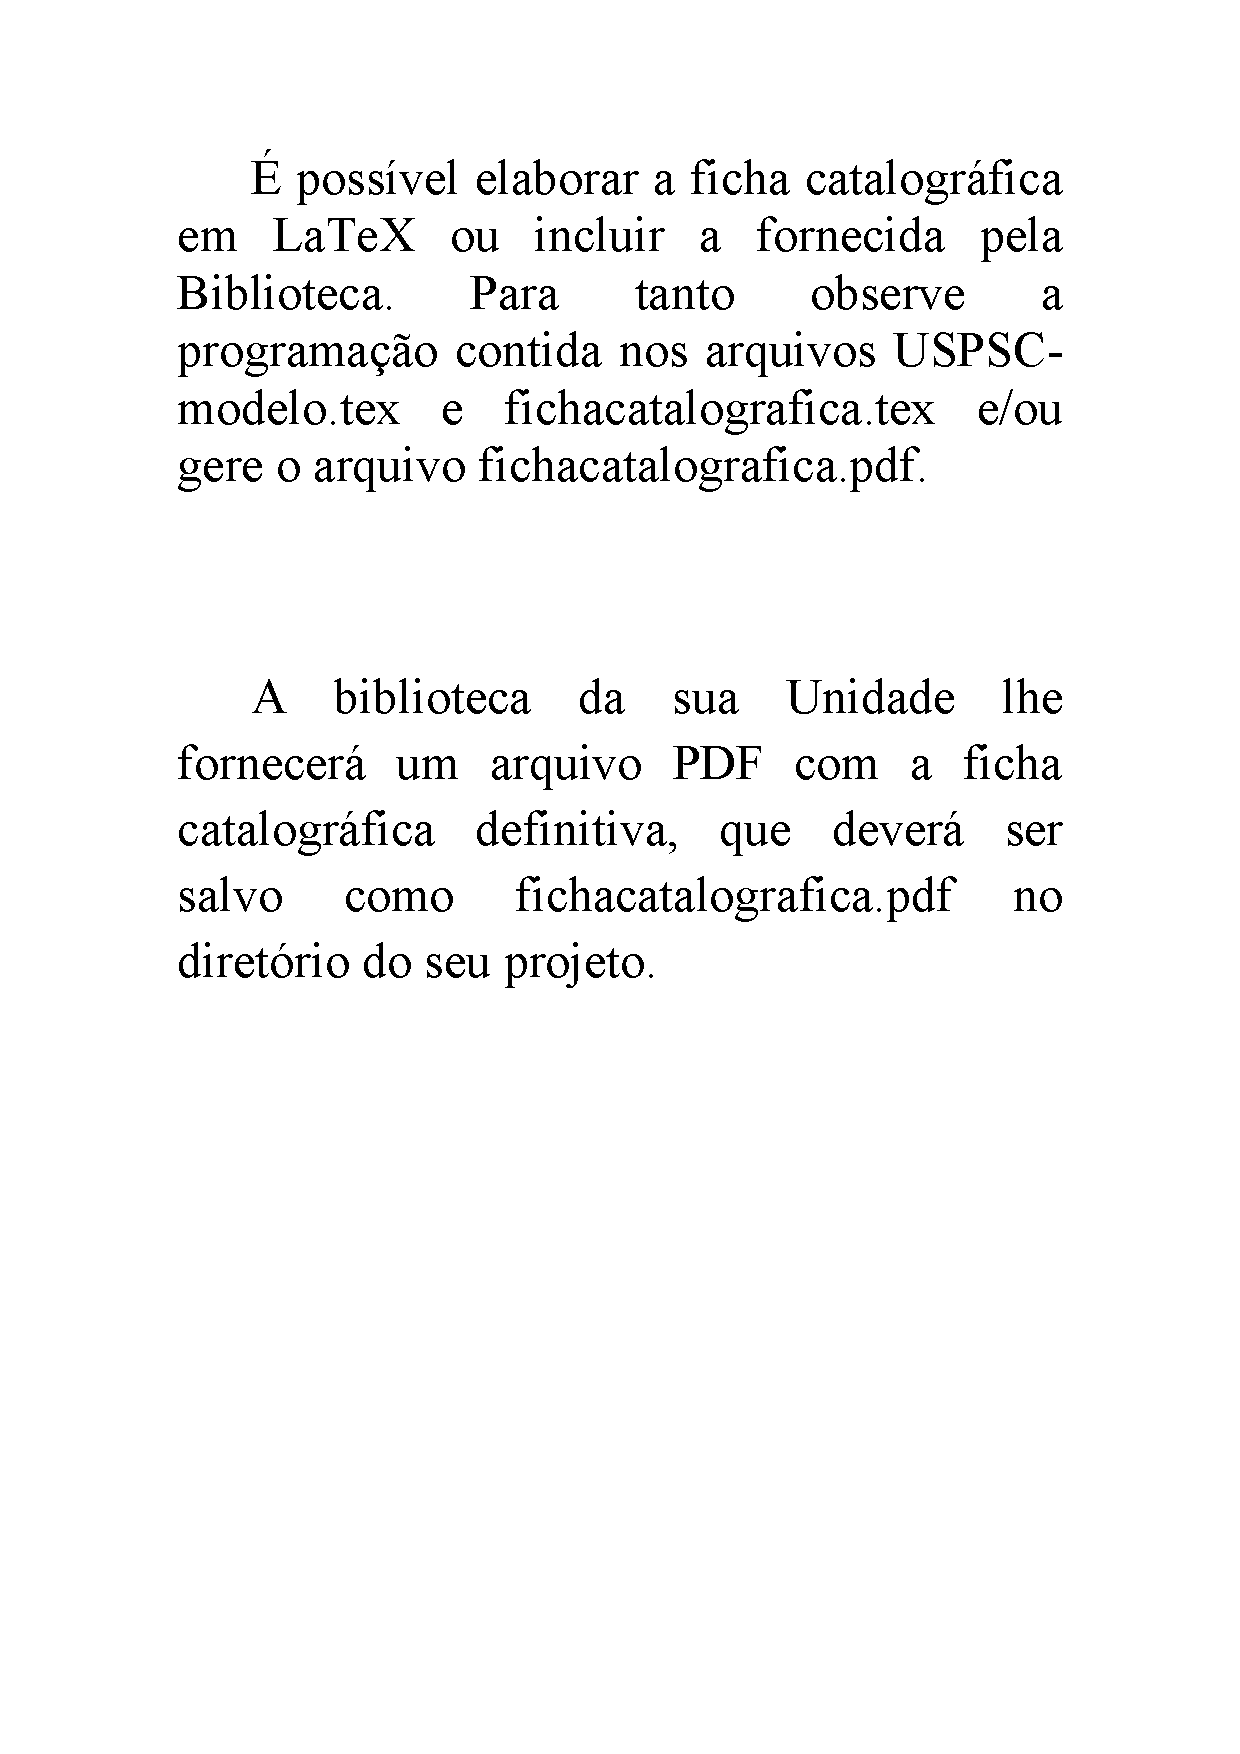
\includepdf{pretextual/USPSC-fichacatalografica.pdf}
    %% USPSC-fichacatalografica.tex
% ---
% Inserir a ficha bibliografica
% ---
% Isto é um exemplo de Ficha Catalográfica, ou ``Dados internacionais de
% catalogação-na-publicação''. Você pode utilizar este modelo como referência. 
% Porém, provavelmente a biblioteca da sua universidade lhe fornecerá um PDF
% com a ficha catalográfica definitiva após a defesa do trabalho. Quando estiver
% com o documento, salve-o como PDF no diretório do seu projeto e substitua todo
% o conteúdo de implementação deste arquivo pelo comando abaixo:
%
\begin{fichacatalografica}
	\hspace{-1.4cm}
	\imprimirnotaautorizacao \\ \\
	%\sffamily
	\vspace*{\fill}					% Posição vertical
\begin{center}					% Minipage Centralizado
  \imprimirnotabib \\
  \begin{table}[htb]
	\scriptsize
	\centering	
	\begin{tabular}{|p{0.9cm} p{8.7cm}|}
		\hline
	      & \\
		  &	  \imprimirautorficha     \\
		
		 \imprimircutter & 
							\hspace{0.4cm}\imprimirtitulo~  / ~\imprimirautor~ ;  ~\imprimirorientadorcorpoficha. -- 	\imprimirlocal, \imprimirdata.   \\
		
		  &  % Para incluir nota referente à versão corrigida no corpo da ficha,
			  % incluir % no início da linha acima e tirar a % do início da linha abaixo
			  %	\hspace{0.4cm} \imprimirtitulo~  / ~\imprimirautor~ ; ~\imprimirorientadorcorpoficha~- ~\imprimirnotafolharosto. -- \imprimirlocal, \imprimirdata.  \\
		
			\hspace{0.4cm}\pageref{LastPage} p. : il. (algumas color.) ; 30 cm.\\ 
		  & \\
		  & 
		    \hspace{0.4cm}\imprimirnotaficha ~--~ 
						  \imprimirunidademin, 
						  \imprimiruniversidademin, 
		                  \imprimirdata. \\ 
		  & \\                 
		   % Para incluir nota referente à versão corrigida em notas,
		    % incluir uma % no início da linha acima e	
		    % tirar a % do início da linha abaixo
		    % & \hspace{0.4cm}\imprimirnotafolharosto \\ 
		  & \\ 
		  & \hspace{0.4cm}1. LaTeX. 2. abnTeX. 3. Classe USPSC. 4. Editoração de texto. 5. Normalização da documentação. 6. Tese. 7. Dissertação. 8. Documentos (elaboração). 9. Documentos eletrônicos. I. \imprimirorientadorficha. 
		   II. Título. \\
	
		     %Se houver co-orientador, inclua % antes da linha (antes de II. Título.) 
		     %          e tire a % antes do comando abaixo 
		     %III. Título. \\   
		  \hline
	\end{tabular}
  \end{table}
\end{center}
\end{fichacatalografica}
% ---



% Folha de rosto adicional
    \imprimirfolhaderostoadic*

% Inserir errata
%%% USPSC-Errata.tex
\begin{errata}
	%\OnehalfSpacing 			
	A errata é um elemento opcional, que consiste de uma lista de erros da obra, precedidos pelas folhas e linhas onde eles ocorrem e seguidos pelas correções correspondentes. Deve ser inserida logo após a folha de rosto e conter a referência do trabalho para facilitar sua identificação, conforme a ABNT NBR 14724 \cite{nbr14724}.
	
	Modelo de Errata:
		
	\begin{flushleft} 
			\setlength{\absparsep}{0pt} % ajusta o espaçamento da referência	
			\SingleSpacing 
			\imprimirautorabr~ ~\textbf{\imprimirtituloresumo}.	\imprimirdata. \pageref{LastPage} p. 
			%Substitua p. por f. quando utilizar oneside em \documentclass
			%\pageref{LastPage} f.
			\imprimirtipotrabalho~-~\imprimirinstituicao, \imprimirlocal, \imprimirdata. 
 	\end{flushleft}
\vspace{\onelineskip}
\OnehalfSpacing 
\center
\textbf{ERRATA}
\vspace{\onelineskip}
\OnehalfSpacing 
\begin{table}[htb]
	\center
	\footnotesize
	\begin{tabular}{p{2cm} p{2cm} p{4cm} p{4cm} }
		\hline
		\textbf{Folha} & \textbf{Linha}  & \textbf{Onde se lê}  & \textbf{Leia-se}  \\
			\hline
			1 & 10 & auto-conclavo & autoconclavo\\
		\hline
	\end{tabular}
\end{table}
\end{errata}
% ---

% Inserir folha de aprovação
% A Folha de aprovação é um elemento obrigatório da NBR 4724/2011 (seção 4.2.1.3).
% 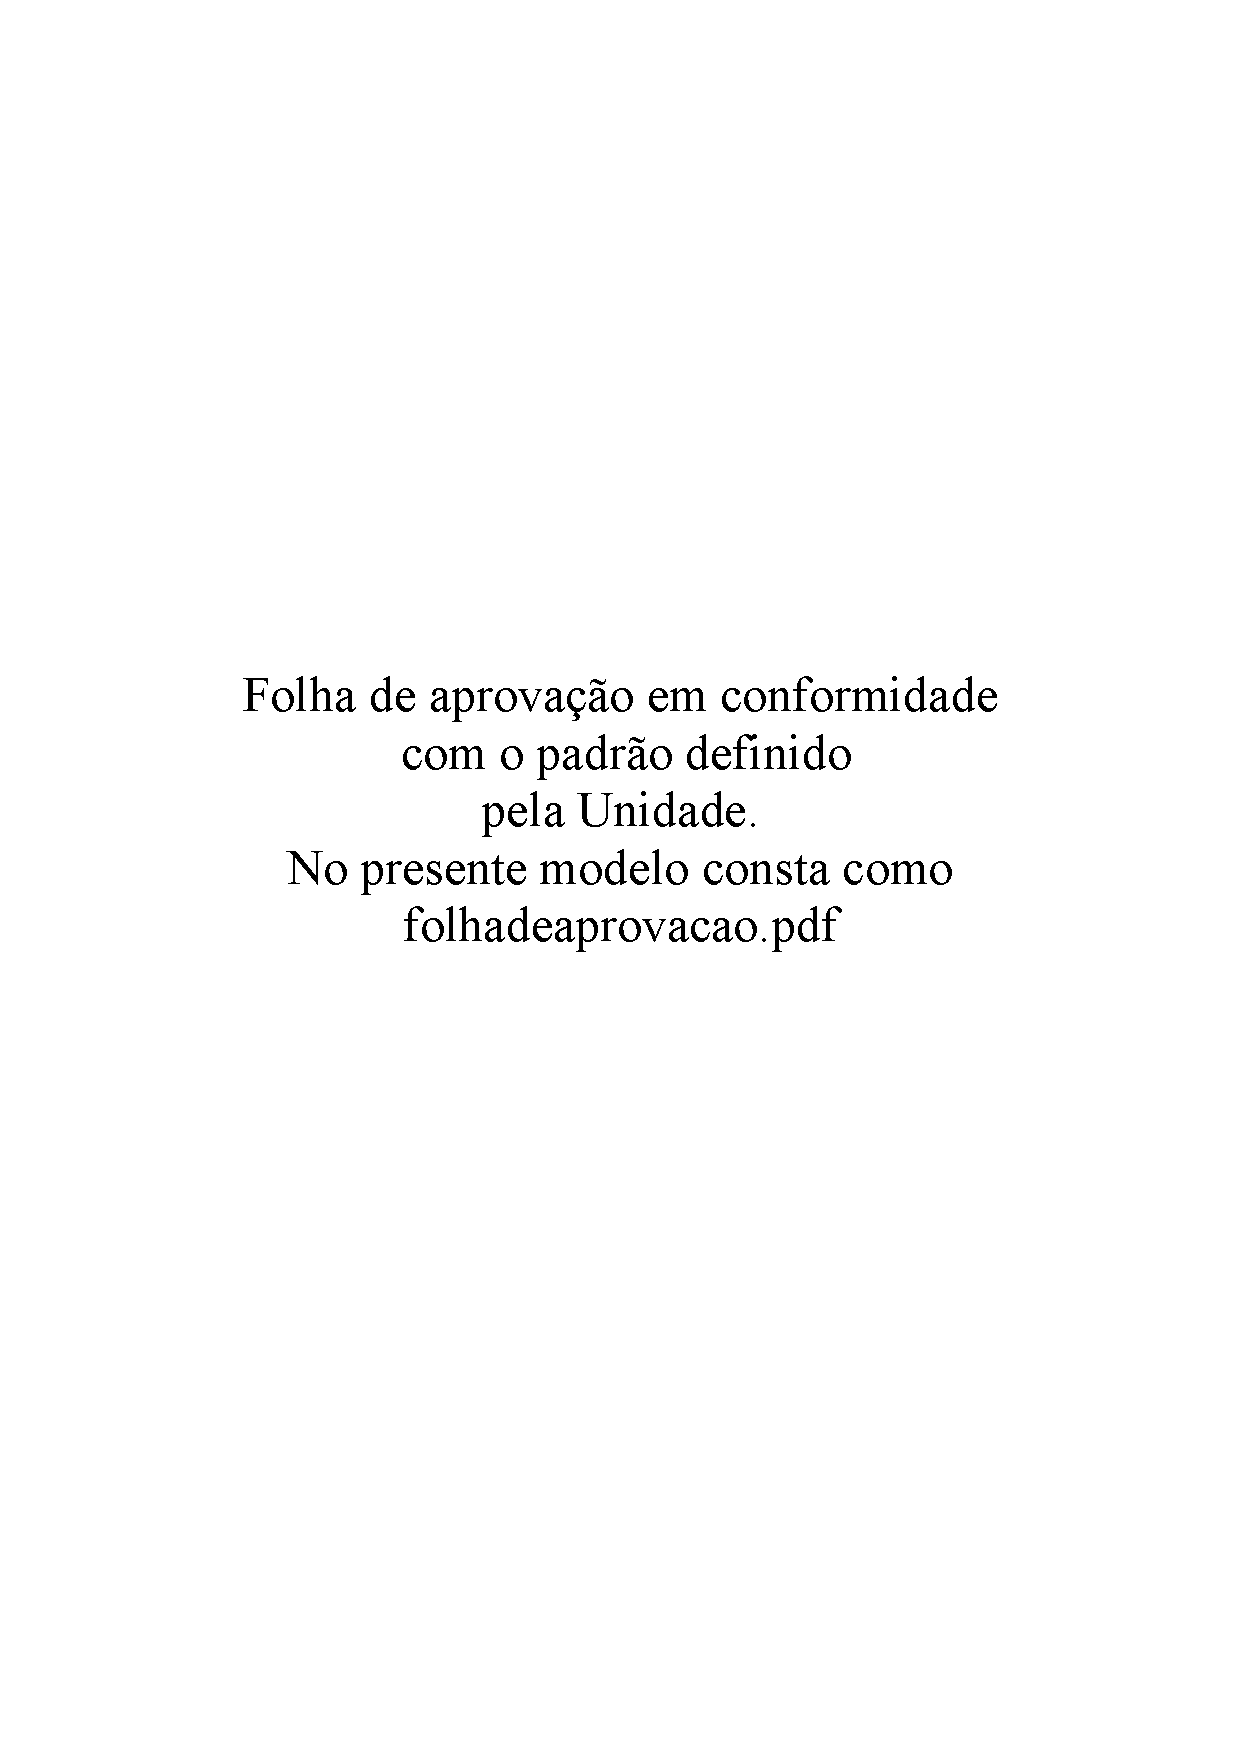
\includepdf{pretextual/USPSC-folhadeaprovacao.pdf}

% Alternativa para a Folha de Aprovação:
%\include{folhadeaprovacao}

% 
\includepdf{pretextual/USPSC-PaginaEmBranco.pdf}
% Dedicatória
%%% USPSC-Dedicatoria.tex
\begin{dedicatoria}
   \vspace*{\fill}
   \centering
   \noindent
   \textit{ Este trabalho é dedicado aos alunos da USP, como uma contribuição\\
  das Bibliotecas do Campus USP de São Carlos para o desenvolvimento\\
	e disseminação da pesquisa científica da Universidade.} \vspace*{\fill}
\end{dedicatoria}
% ---

% Agradecimentos
%%% USPSC-Agradecimentos.tex
\begin{agradecimentos}
	Primeira frase do agradecimento ....
	
	Segunda frase ....
	
	Outras frases ....
	
	Última frase ....
	
\end{agradecimentos}
% ---

% Epígrafe
%%% USPSC-Epigrafe.tex
\begin{epigrafe}
    \vspace*{\fill}
	\begin{flushright}
		\textit{``O estudo, a busca da verdade e da beleza são domínios \\
		em que nos é consentido sermos crianças por toda a vida.''\\
		Albert Einstein}
	\end{flushright}
\end{epigrafe}
% ---

% Se o idioma do texto for em inglês, o abstract deve preceder o resumo em português

% Abstract
    %% USPSC-Abstract.tex
%\autor{Silva, M. J.}
\begin{resumo}[Abstract]
 \begin{otherlanguage*}{english}
	\begin{flushleft} 
		\setlength{\absparsep}{0pt} % ajusta o espaçamento dos parágrafos do resumo		
 		\SingleSpacing  		\imprimirautorabr~~\textbf{\imprimirtitleabstract}.	\imprimirdata.  \pageref{LastPage} p. 
		%Substitua p. por f. quando utilizar oneside em \documentclass
		%\pageref{LastPage} f.
		\imprimirtipotrabalhoabs~-~\imprimirinstituicao, \imprimirlocal, 	\imprimirdata. 
 	\end{flushleft}
	\OnehalfSpacing 
   This is the english abstract.

   \vspace{\onelineskip}
 
   \noindent 
   \textbf{Keywords}: LaTeX. USPSC class. Thesis. Dissertation. Conclusion course paper. Report. 
 \end{otherlanguage*}
\end{resumo}

    %% USPSC-Resumo.tex
\setlength{\absparsep}{18pt} % ajusta o espaçamento dos parágrafos do resumo		
\begin{resumo}
	\begin{flushleft} 
			\setlength{\absparsep}{0pt} % ajusta o espaçamento da referência	
			\SingleSpacing 
			\imprimirautorabr~~\textbf{\imprimirtituloresumo}.	\imprimirdata. \pageref{LastPage} p. 
			%Substitua p. por f. quando utilizar oneside em \documentclass
			%\pageref{LastPage} f.
			\imprimirtipotrabalho~-~\imprimirinstituicao, \imprimirlocal, \imprimirdata. 
 	\end{flushleft}
\OnehalfSpacing 			
 O resumo deve ressaltar o  objetivo, o método, os resultados e as conclusões do documento.
 A ordem e a extensão  destes itens dependem do tipo de resumo (informativo ou indicativo) e do tratamento que cada item recebe no documento original.
 O resumo deve ser precedido da referência do documento, com exceção do resumo inserido no próprio documento. (\ldots)
	Salientamos que algumas Unidades exigem o titulo dos trabalhos acadêmicos em inglês,
	tornando necessário a inclusão das referências nos resumos e abstracts,
	o que foi adotado no \textbf{Modelo para TCC em \LaTeX\ utilizando a classe USPSC} e no
	\textbf{Modelo para teses e dissertações em \LaTeX\ utilizando a classe USPSC}.
	As palavras-chave devem figurar logo abaixo do  resumo, antecedidas da expressão Palavras-chave:,
	separadas entre si por  ponto e finalizadas também por ponto \cite{nbr6028}.
 

 \textbf{Palavras-chave}: LaTeX. Classe USPSC. Tese. Dissertação. Trabalho de conclusão de curso (TCC). Relatório.
\end{resumo}

% inserir lista de figurass
%\pdfbookmark[0]{\listfigurename}{lof}
%\listoffigures*
%\cleardoublepage

% inserir lista de tabelas
%\pdfbookmark[0]{\listtablename}{lot}
%\listoftables*
%\cleardoublepage

% inserir lista de quadros
%\pdfbookmark[0]{\listofquadroname}{loq}
%\listofquadro*
%\cleardoublepage

% inserir lista de abreviaturas e siglas
%% USPSC-AbreviaturasSiglas.tex
\begin{siglas}
    \item[ABNT] Associação Brasileira de Normas Técnicas
    \item[abnTeX] ABsurdas Normas para TeX
	\item[IBGE] Instituto Brasileiro de Geografia e Estatística
	\item[LaTeX] Lamport TeX
	\item[USP] Universidade de São Paulo
	\item[USPSC] Campus USP de São Carlos
\end{siglas}


% inserir lista de símbolos
%% USPSC-Simbolos.tex
\begin{simbolos}
  \item[$ \Gamma $] Letra grega Gama
  \item[$ \Lambda $] Lambda
  \item[$ \zeta $] Letra grega minúscula zeta
  \item[$ \in $] Pertence
\end{simbolos}

% inserir o sumario
    \pdfbookmark[0]{\contentsname}{toc}
    \tableofcontents*
    \cleardoublepage

% ----------------------------------------------------------
% ELEMENTOS TEXTUAIS
% ----------------------------------------------------------
    \textual

% Capítulo 1 - Introdução
    \chapter{Introdução}

O livro de ordens limite representa o estado atual de todas ordens aguardando execução. Essencialmente fornece uma representação dinâmica das intenções de compra e venda de ativos financeiros em um determinado mercado por meio de uma lista de ordens, ordenadas por preço e tempo de chegada, onde cada entrada representa o desejo de um participante do mercado de comprar ou vender um certo ativo \citep{Abergel2020, Avellaneda2008}. Os intervalos de tempo entre a chegada de duas ordens subsequentes são comumente representados por processos estocásticos e o estudo desses processos é uma abordagem fundamental para a modelagem e representação da dinâmica dos mercados financeiros \citep{Shi2022, Guilbaud2013, Liu2021}. Tradicionalmente, os modelos de chegada de ordens têm se baseado em processos de contagem, onde os incrementos entre eventes são distribuídos de acordo com distribuições de Poisson ou distribuições exponenciais \citep{Cont2022, Ponta2012}. Recentemente surge grande interesse na utilização de processos de Hawkes para modelar os processos de chegada, devido a natureza autoexcitável dos mesmos \citep{Abergel2020, MorariuPatrichi2022, Toke2011}. 

O uso de uma distribuição com parâmetros fixos para estimar os tempos de chegada não considera as diferentes propriedades dentre os diversos regimes financeiros existentes do mercado, tanto em escala macro, como por exemplo regimes de inflação \citep{Krause2022}, como em escalas de curto prazo, como por exemplo regimes de alta ou baixa volatilidade, liquidez e volume de negociação \citep{Guilbaud2013}, que exibem comportamentos distintos entre si. Esses regimes podem ser influenciados por uma variedade de fatores, incluindo eventos econômicos, políticos e sazonais e resultam em alterações nas características estatísticas dos processos de preços, e chegada de ordens \citep{Krause2022}.

Uma abordagem promissora que considere os efeitos dos diferentes regimes é o uso de modelos ocultos de Markov (\textit{Hidden Markov Chains}, em inglês, ou \textit{HMC}) \citep{Cont2010}. Um \textit{HMC} é um modelo estocástico que assume a existência de estados ocultos, não observáveis diretamente, mas que podem ser inferidos a partir de observações de variáveis externas \citep{Baum1966}. Nesse contexto, os diferentes estados ou regimes implícitos do livro de ordens e as diferentes intensidades de chegada de ordens podem ser representados como estados ocultos da cadeia de Markov e as distribuições ou parâmetros associados com os respectivos estados \citep{MorariuPatrichi2022}. Essa abordagem permite modelar a transição entre diferentes regimes de mercado de forma dinâmica, considerando uma matriz de transição de estados.

Na literatura de simulação de livros de ordem foram utilizados alguns modelos para a identificação e simulação dos diferentes estados do livro, como por exemplo modelos de \textit{Markov Switching} \citep{Guilbaud2013} ou algoritmos de \textit{Thinning} para simulação de processos dependentes de estados \citep{Ponta2012}. Além disso, as distribuições utilizadas para modelar o processo de chegada de ordens são mantidas fixas durante a simulação, com apenas seus parâmetros sendo ajustados e obtidos a partir dos estados atuais. Em suma, essas abordagens requerem que sejam feitas assunções sobre o funcionamento intrínsico do mercado, além de limitar as características estatísticas da simulação apenas ao período observado devido ao ajuste dos parâmetros não capturarem todas características do conjunto de dados \citep{Zare2021}.

Considerando tais problemas, o presente trabalho propõe o uso e comparação de duas abordagens numéricas para otimizar a amostragem das distribuições dos processos de chegada, cujo formato é tomado como desconhecido como ponto de partida inicial: 
\begin{itemize}
	\item Algoritmos genéticos (AGs) têm se destacado como uma ferramenta poderosa para otimização e modelagem em uma variedade de domínios, incluindo finanças \citep{Oesch2013, Katoch2021}. Esses algoritmos podem ser aplicados para aproximar as possíveis distribuições dos processos de chegada de ordens, utilizando estimativas por máxima verossimilhança \citep{Boonthiem2023, Colla2010} para ajustar os parâmetros das populações aos dados históricos observados;
	
	\item Métodos de Monte Carlo para Cadeias de Markov (\textit{Markov chain Monte Carlo } em inglês, ou MCMC) também vêm ganhando destaque como uma abordagem eficaz para amostragem de distribuições complexas e multidimensionais \citep{Rasmussen2013, Rousseau2018}. Os métodos de MCMC, como o algoritmo de Metropolis-Hastings e o Gibbs sampling, são particularmente úteis quando se trata de amostrar a partir de distribuições de probabilidade desconhecidas ou difíceis de obter diretamente \citep{Glasserman2004}. Ao construir uma cadeia de Markov com distribuição estacionária igual à distribuição alvo, esses métodos podem possivelmente gerar amostras que representam fielmente a distribuição desejada.
\end{itemize}

Em suma, este trabalho propõe uma abordagem computacional alternativa para modelar e simular o livro de ordens limite e os processos de chegada de ordens no mercado financeiro, utilizando Hidden Markov Chains e otimizadores de amostragens por meio de bibliotecas de computação em unidades de processamento gráficas (\textit{GPUs}). As abordagens propostas tem o potencial de melhorar significativamente a precisão das simulações e fornecer propriedades estatísticas mais robustas sobre o comportamento do mercado em diferentes regimes para teste de estratégias de negociação algorítmicas.


% Capítulo 2
    %% USPSC-Cap2-Desenvolvimento.tex 

% ---
% Este capítulo, utilizado por diferentes exemplos do abnTeX2, ilustra o uso de
% comandos do abnTeX2 e de LaTeX.
% ---

\chapter{Development}
\label{ch:development}
%Este capítulo é parte principal do trabalho acadêmico e deve conter a exposição ordenada e detalhada do assunto.
%Divide-se em seções e subseções, em conformidade com a abordagem do tema e do método, abrangendo:
%revisão bibliográfica, materiais e métodos, técnicas utilizadas, resultados obtidos e discussão.

Distributed reinforcement learning (RL) has evolved considerably in response to the demands of complex tasks such as game playing and financial trading.
Early methods such as the Asynchronous Advantage Actor-Critic (A3C)
algorithm introduced the concept of multiple parallel workers collecting experiences independently,
which helped to reduce update variance and speed up training.
Building on these ideas, architectures like IMPALA have decoupled data collection from model training by deploying a
centralized learner that periodically synchronizes its policy with a large number of worker agents.
This design enables significant scalability across heterogeneous computing resources and facilitates high-throughput training.

A key challenge addressed by these systems is the communication overhead incurred when transmitting experiences and
updated policies between the learner and the workers.
For example, IMPALA aggregates trajectories from multiple workers into
batches for efficient gradient computation while managing the staleness of policy information.
More recent approaches, such as SEED RL, have further optimized communication by bundling inference with training updates.
This reduces the latency associated with model parameter transmission and minimizes network congestion, thereby improving overall training efficiency.
In parallel, methods like Ape-X have introduced distributed prioritized experience replay, where critical experiences are sampled with higher probability,
enhancing data efficiency in scenarios where high-frequency data generation is crucial.

In the context of financial applications, distributed RL has inspired specialized solutions that integrate realistic market simulators.
These simulators often feature a limit order book (LOB) mechanism where buy and sell orders are submitted, queued, and matched in real time.
In such systems, the distributed architecture must handle not only the high throughput of simulation data but also the
precise timing of order execution and asynchronous policy updates.
Recent studies have demonstrated that merging shared environment simulations with asynchronous updates can improve both
computational efficiency and learning performance in trading scenarios.

Despite these advances, challenges persist—such as managing synchronization delays, mitigating data staleness,
and coping with non-stationarity—especially in environments where rapid decision making is essential.
The trade-offs between synchronous and asynchronous communication, efficient use of replay buffers, and resource heterogeneity remain open research questions.
This thesis builds upon these existing approaches by proposing a novel shared parallel environment architecture,
designed specifically to address these challenges in high-frequency trading applications.
In the following sections, we present the design and implementation of our proposed architecture,
which we refer to as the Parallel Environments for Asynchronous Reinforcement Learning (PEARL).

We start with an overview of related works in distributed RL and financial trading, followed by a detailed description of the PEARL architecture.

\section{Literature Review}
\label{sec:literature_review}

We performed a simple overview of recent literature regarding distributed reinforcement learning,
and categorized the results according to groups of tags.
This review was made with the purpose of highlighting frequently used algorithms, RL metrics,
and types of system and network benchmarks.
To gather relevant literature, we searched the Web of Science database using the following search query,
while limiting the results to the last 5 years:

\begin{verbatim}
    ALL=(
        (
            "distributed" OR "parallel" OR
            "multi-agent" OR "asynchronous"
        )
        AND
        (
            "shared environments" OR "replay buffer" OR
            "trajectory sampling" OR "experience sampling"
        )
        AND "reinforcement learning"
    )
\end{verbatim}

Initially, a total of 68 papers matched the search query, with 34 being deemed unfit or irrelevant to the
present research question.
The bibliography analysis refeers to the remaining 33, where the tagged categories are as shown:

\begin{itemize}[leftmargin=*, label={--}]
    \item \textbf{Algorithm Categories} (e.g., Q-learning, Actor-Critic, Policy Gradients)
    \item \textbf{Learning Paradigm} (On-Policy, Off-Policy, Model-Free, Model-Based)
    \item \textbf{Communication Model} (Centralized, Decentralized, Asynchronous, Synchronous)
    \item \textbf{RL Metrics} (Reward, Sample Efficiency, Convergence, Stability)
    \item \textbf{System Metrics} (Wall Speed, Latency, Memory, Core Efficiency)
\end{itemize}



\section{Methodology}
\label{sec:methodology}

This thesis makes several key contributions to the field of distributed reinforcement learning by introducing a novel shared
parallel environment architecture that addresses common inefficiencies in traditional systems.
Our approach, called Parallel Environments for Asynchronous Reinforcement Learning (PEARL),
is designed to enhance computational efficiency and learning performance in high-frequency trading applications.

First, the proposed framework enables multiple RL agents (workers) to share a single environment instance rather than running isolated simulations.
This design minimizes redundant computations and significantly reduces the communication overhead typically
encountered when synchronizing  separate environment instances.
Second, the system incorporates an asynchronous policy update mechanism.
In our approach, workers continuously send their experience trajectories to a centralized learner without waiting for all processes to complete,
thereby mitigating issues of data staleness and enhancing convergence stability in non-stationary environments

Third, we validate the proposed architecture within the context of financial applications,
such as high-frequency trading, demonstrating that the shared environment
model can achieve superior computational efficiency and learning performance compared to conventional actor-learner designs.

\subsection{Simulated Trading Environment and Limit Order Book Dynamics}

The simulated environment is designed to replicate key aspects of a modern financial market by incorporating a limit order book (LOB) mechanism.
A LOB is the core structure in many electronic trading systems, where buy and sell orders are organized by price and time priority,
thereby reflecting the real-time supply and demand of an asset.

In this environment, agents interact with the market by submitting orders that represent their actions.
Specifically, each action corresponds to placing a limit order—a directive to buy or sell a specified quantity at a predetermined price.
When an agent submits an order, it is added to the appropriate side of the LOB, where orders are queued according to their price and
the time at which they were submitted.
An order is executed if there is a matching order on the opposite side of the book that satisfies the price condition;
otherwise, it remains in the book until a suitable counter-order appears or the order is cancelled by the agent.
This event-driven process mimics the intricate dynamics of order matching observed in real markets.

The simulation employs a discrete-event framework to model these processes accurately.
At each simulation step, the environment generates an observation that includes critical details such as the best bid and ask prices,
the order book depth across various price levels, and records of recent trade executions.
These observations are then provided to the agents, enabling them to update their strategies based on the evolving market state.

Order submission and execution in the simulated environment are handled asynchronously.
Agents send their orders via a messaging layer—implemented with a high-performance protocol like
ZeroMQ—to ensure that multiple agents can interact with the shared LOB concurrently without incurring significant delays.
This asynchronous architecture not only improves simulation throughput but also closely aligns with
the latency-sensitive nature of high-frequency trading environments.

By integrating a realistic LOB into the simulation, the environment provides a robust testbed for exploring how
distributed reinforcement learning algorithms can learn and adapt in complex, dynamic markets.
The detailed representation of market microstructure, combined with the precise handling of order events,
allows for rigorous scientific investigation into the interplay between order submission strategies and market behavior.


\subsection{Parallel Environments for Asynchronous Reinforcement Learning (PEARL)}

The proposed architecture builds on the core idea of sharing a single, highly parallel environment among multiple agents while
maintaining an efficient and scalable actor–learner framework.
In contrast to conventional distributed reinforcement learning systems—where each worker simulates an independent environment instance—
the shared environment paradigm leverages a unified simulation that is concurrently accessed by multiple workers.
This design minimizes redundant computations and memory overhead,
which is especially critical in high-frequency trading simulations where the fidelity and speed of the limit order book (LOB) dynamics are paramount.

At the heart of the architecture lies a central learner that manages the global policy.
Upon initialization, the learner spawns several worker processes using a framework such as Ray.
Each worker retrieves the latest version of the shared policy and uses it to interact with the common environment.
In this setup, workers act as both data collectors and order executors: they send orders (actions) to the LOB simulation,
receive market updates, and construct trajectories that capture the sequence of states, actions, and rewards.
By sharing the environment, workers benefit from a consistent and synchronized view of the simulated market,
which enhances the quality of the experience data collected.

Communication between the learner and workers is designed to be asynchronous.
Workers submit their generated trajectories to the learner via a high-performance messaging layer implemented with ZeroMQ.
This asynchronous mechanism enables workers to operate independently—without waiting for policy updates—
thereby reducing idle time and mitigating the staleness issues often encountered in distributed setups

). Meanwhile, the learner continuously processes incoming trajectories from the workers, updates the global policy using reinforcement learning algorithms,
and periodically broadcasts the refined policy back to the workers.
This cycle ensures that while each worker may temporarily operate on slightly outdated policy parameters,
the overall system converges steadily as fresh data are incorporated into the learner's updates.

The integration of Ray not only facilitates parallel process management but also supports dynamic resource allocation.
By abstracting the complexities of distributed computing, Ray allows the system to scale horizontally across multiple nodes,
ensuring that the computational load—especially during intensive simulations and gradient computations—is balanced effectively.
This scalability is crucial when simulating environments with rapidly changing market conditions,
where the ability to quickly process large volumes of data directly translates into more effective learning

Furthermore, the unified communication protocol and shared environment design contribute to reducing the overall system latency.
In traditional architectures, the cost of transferring model parameters and simulation data between isolated environment instances can
introduce significant delays. By contrast, our approach minimizes such overhead by centralizing the simulation and leveraging efficient,
low-latency communication channels.
This architecture is particularly well-suited for real-time applications, such as high-frequency trading,
where even minor delays can adversely affect performance

In summary, this integrated system architecture—comprising a shared simulation environment, an asynchronous actor–learner framework, and
a robust communication backbone—addresses many of the limitations inherent in earlier distributed reinforcement learning approaches.
By combining the advantages of shared resource utilization with scalable, asynchronous updates, the architecture provides a solid foundation for
developing reinforcement learning systems capable of operating effectively in complex, dynamic domains.


\section{Technical Details and Framework Description}
\label{sec:technical_details}


%\begin{table}[H]
%\begin{table}[htb]
%	\IBGEtab{%
%		\caption{Frequência anual por categoria de usuários}%
%		\label{tab-ibge}
%	}{%
%		\begin{tabular}{ccc}
%			\toprule
%			Categoria de Usuários & Frequência de Usuários \\
%			\midrule \midrule
%			Graduação & 72\% \\
%			\midrule
%			Pós-Graduação & 15\% \\
%			\midrule
%			Docente & 10\% \\
%			\midrule
%			Outras & 3\% \\
%			\bottomrule
%		\end{tabular}%
%	}{%
%		\fonte{Elaborada pelos autores.}%
%		\nota{Exemplo de uma nota.}%
%		\nota[Anotações]{Uma anotação adicional, que pode ser seguida de várias
%			outras.}%
%
%	}
%\end{table}

%
%A formatação do quadro é similar à tabela, mas deve ter suas laterais fechadas e conter as linhas horizontais.
%\newpage

% o comando \newpage foi utilizado para forçar a quebra de página

%\begin{quadro}[htb]
%	\caption{\label{quadro_modelo}Níveis de investigação}
%	\begin{tabular}{|p{2.6cm}|p{6.0cm}|p{2.25cm}|p{3.40cm}|}
%		\hline
%		\textbf{Nível de Investigação} & \textbf{Insumos}  & \textbf{Sistemas de Investigação}  & \textbf{Produtos}  \\
%		\hline
%		Meta-nível & Filosofia\index{filosofia} da Ciência  & Epistemologia &
%		Paradigma  \\
%		\hline
%		Nível do objeto & Paradigmas do metanível e evidências do nível inferior &
%		Ciência  & Teorias e modelos \\
%		\hline
%		Nível inferior & Modelos e métodos do nível do objeto e problemas do nível inferior & Prática & Solução de problemas \\
%		\hline
%	\end{tabular}
%	\begin{flushleft}
%		%\fonte{\citeonline{van1986}}
%		Fonte: \citeonline{van1986}
%	\end{flushleft}
%\end{quadro}


%% ---
%\subsection{Figuras}\label{sec_figuras}
%% ---
%\index{figuras}Figuras podem ser criadas diretamente em \LaTeX,
%como o exemplo da \autoref{fig_circulo}.

%\begin{figure}[htb]
%	\caption{\label{fig_circulo}A delimitação do espaço}
%	\begin{center}
%		\setlength{\unitlength}{9cm}
%		\begin{picture}(1,1)
%		\put(0,0){\line(0,1){1}}
%		\put(0,0){\line(1,0){1}}
%		\put(0,0){\line(1,1){1}}
%		\put(0,0){\line(1,2){.5}}
%		\put(0,0){\line(1,3){.3333}}
%		\put(0,0){\line(1,4){.25}}
%		\put(0,0){\line(1,5){.2}}
%		\put(0,0){\line(1,6){.1667}}
%		\put(0,0){\line(2,1){1}}
%		\put(0,0){\line(2,3){.6667}}
%		\put(0,0){\line(2,5){.4}}
%		\put(0,0){\line(3,1){1}}
%		\put(0,0){\line(3,2){1}}
%		\put(0,0){\line(3,4){.75}}
%		\put(0,0){\line(3,5){.6}}
%		\put(0,0){\line(4,1){1}}
%		\put(0,0){\line(4,3){1}}
%		\put(0,0){\line(4,5){.8}}
%		\put(0,0){\line(5,1){1}}
%		\put(0,0){\line(5,2){1}}
%		\put(0,0){\line(5,3){1}}
%		\put(0,0){\line(5,4){1}}
%		\put(0,0){\line(5,6){.8333}}
%		\put(0,0){\line(6,1){1}}
%		\put(0,0){\line(6,5){1}}
%		\end{picture}
%	\end{center}
%	\legend{Fonte: \citeonline{equipeabntex2}}
%\end{figure}

%Isto é uma \texttt{subsubsection} do \LaTeX, mas é denominada de ``subseção'' porque no português não temos a palavra ``subsubseção''.

%\paragraph{Este é um parágrafo numerado}\label{sec-exemplo-paragrafo}

%\begin{verbatim}
%\paragraph{Este é um parágrafo numerado}\label{sec-exemplo-paragrafo}
%\end{verbatim}









% Capítulo 4 - Conclusão
    %% USPSC-Cap3-Conclusao.tex
% ---
% Conclusão
% ---
\chapter{Conclusion}
\label{ch:conclusion}
% ---
% O comando abaixo insere parágrafos aleatórios só para exemplificar
%Apresentar as conclusões correspondentes aos objetivos ou hipóteses propostos para o desenvolvimento do trabalho, podendo incluir sugestões para novas pesquisas.



% ----------------------------------------------------------
% ELEMENTOS PÓS-TEXTUAIS
% ----------------------------------------------------------
    \postextual

% Referências bibliográficas
%\bibliography{USPSC-bib/uspbib}
    \bibliography{bib/bibliograpy}

% Glossário
%\glossary

% Apêndices
%%% USPSC-Apendice.tex
% ---
% Inicia os apêndices
% ---

\begin{apendicesenv}
% Imprime uma página indicando o início dos apêndices
\partapendices
\chapter{apêndice(s)}
Elemento opcional, que consiste em texto ou documento elaborado pelo autor, a fim de complementar sua argumentação, conforme a ABNT NBR 14724 \cite{nbr14724}.

Os apêndices devem ser identificados por letras maiúsculas consecutivas, seguidas de hífen e pelos respectivos títulos. Excepcionalmente, utilizam-se letras maiúsculas dobradas na identificação dos apêndices, quando esgotadas as 26 letras do alfabeto. A paginação deve ser contínua, dando seguimento ao texto principal. \cite{aguia2020}
% ----------------------------------------------------------
\chapter{Exemplo de tabela centralizada verticalmente e horizontalmente}
\index{tabelas}A \autoref{tab-centralizada} exemplifica como proceder para obter uma tabela centralizada verticalmente e horizontalmente.
% utilize \usepackage{array} no PREAMBULO (ver em USPSC-modelo.tex) obter uma tabela centralizada verticalmente e horizontalmente
\begin{table}[htb]
\ABNTEXfontereduzida
\caption[Exemplo de tabela centralizada verticalmente e horizontalmente]{Exemplo de tabela centralizada verticalmente e horizontalmente}
\label{tab-centralizada}

\begin{tabular}{ >{\centering\arraybackslash}m{6cm}  >{\centering\arraybackslash}m{6cm} }
\hline
 \centering \textbf{Coluna A} & \textbf{Coluna B}\\
\hline
  Coluna A, Linha 1 & Este é um texto bem maior para exemplificar como é centralizado verticalmente e horizontalmente na tabela. Segundo parágrafo para verificar como fica na tabela\\
  Quando o texto da coluna A, linha 2 é bem maior do que o das demais colunas  & Coluna B, linha 2\\
\hline
\end{tabular}
\begin{flushleft}
		Fonte: Elaborada pelos autores.\
\end{flushleft}
\end{table}

% ----------------------------------------------------------
\chapter{Exemplo de tabela com grade}
\index{tabelas}A \autoref{tab-grade} exemplifica a inclusão de traços estruturadores de conteúdo para melhor compreensão do conteúdo da tabela, em conformidade com as normas de apresentação tabular do IBGE.
% utilize \usepackage{array} no PREAMBULO (ver em USPSC-modelo.tex) obter uma tabela centralizada verticalmente e horizontalmente
\begin{table}[htb]
\ABNTEXfontereduzida
\caption[Exemplo de tabelas com grade]{Exemplo de tabelas com grade}
\label{tab-grade}
\begin{tabular}{ >{\centering\arraybackslash}m{8cm} | >{\centering\arraybackslash}m{6cm} }
\hline
 \centering \textbf{Coluna A} & \textbf{Coluna B}\\
\hline
  A1 & B1\\
\hline
  A2 & B2\\
\hline
  A3 & B3\\
\hline
  A4 & B4\\
\hline
\end{tabular}
\begin{flushleft}
		Fonte: Elaborada pelos autores.\
\end{flushleft}
\end{table}


\end{apendicesenv}
% ---

% Anexos
%%% USPSC-Anexos.tex
% ---
% Inicia os anexos
% ---
\begin{anexosenv}

% Imprime uma página indicando o início dos anexos
\partanexos

% ---
\chapter{Exemplo de anexo}
% ---
Elemento opcional, que consiste em um texto ou documento não elaborado pelo autor, que serve de fundamentação, comprovação e ilustração, conforme a ABNT NBR 14724. \cite{nbr14724}.

O \textbf{ANEXO B} exemplifica como incluir um anexo em pdf.

\chapter{Acentuação (modo texto - \LaTeX)}
\begin{figure}[H]
	\begin{center}
	\caption{\label{fig_anexob}Acentuação (modo texto - \LaTeX)}
	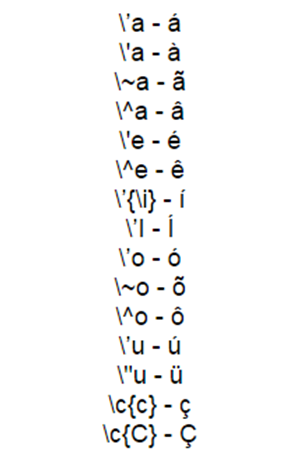
\includegraphics[scale=1.0]{USPSC-img/USPSC-AcentuacaoLaTeX.png} \\
	%Fonte: \citeonline{comandos}
	Fonte: Comandos [\ldots]  (\citeyear{comandos})
	\end{center}	
\end{figure}

\end{anexosenv}


% INDICE REMISSIVO
%%% USPSC-IndicexRemissivos.tex
% ---
% Inicia os Índices Remissivos
% ---
%---------------------------------------------------------------------
% INDICE REMISSIVO
%--------------------------------------------------------------------
\phantompart
\printindex
%---------------------------------------------------------------------


\end{document}
